\documentclass{article}
\usepackage[french]{babel}
\usepackage[a4paper,top=2cm,bottom=2cm,left=3cm,right=3cm,marginparwidth=1.75cm]{geometry}
\usepackage{amsmath}
\usepackage[T1]{fontenc}
\usepackage{graphicx}
\usepackage[colorlinks=true, allcolors=blue]{hyperref}
\DeclareUnicodeCharacter{2082}{$_2$}

\title{L'implication éthique liée à la création de logiciels}
\author{Lynne Guizani, Sephora Mavitidi Bunga, Andrea Lafarge, Bercy Yola}

\begin{document}
\maketitle

\section{Introduction}
L'implication de l'éthique dans la création de logiciels est importante pour notre sécurité et bien-être, mais qu'est-ce que l'éthique ? C'est tout simplement notre sens moral, ce qui nous constitue et nous aide à déterminer ce qui est bien ou mal, dans la création de logiciels, ce sera à propos de la protection des données et l'accessibilité pour les utilisateurs.
\\\\
Pour ce faire, nous allons aborder quatre parties dont certaines directement liées:
Yola commencera par parler des dangers puis d'une infime partie de la loi informatique et liberté, elle sera suivie par Lynne qui abordera la partie environnementale et les droits des travailleurs, ensuite Sephora parlera des problèmes d'accessibilités pour les personnes en situations d'handicap et enfin nous finirons avec Andrea et la protection des données personnelles. 


\subsection{Les lois mises en rigueur et les dangers d'un manque d'éthique dans la création de logiciels (Yola)}

Un problème d'éthique dans le code d'un logiciel peut entraîner le non-respect des lois.\\\\
Par exemple l'IA COMPAS utilisée un temps dans les tribunaux Américains n'aurait jamais pu être mise en place en France car à la suite de recherches, nous avons appris que cette IA portait atteinte à l'identité de certaines personnes, ce qui est non conforme au premier article de la loi relative à l'informatique, aux fichiers et aux libertés dont je parlerai pendant l'entièreté de cette partie.\\\\
En effet cette IA qui devait calculer le taux de possible récidive des condamnés semblait être entraînée à donner un score de récidive plus élevé aux personnes noires qu’aux personnes blanches bien que les mêmes types de profils soient identifiés pour les deux groupes.
\begin{figure}[h]
    \centering
    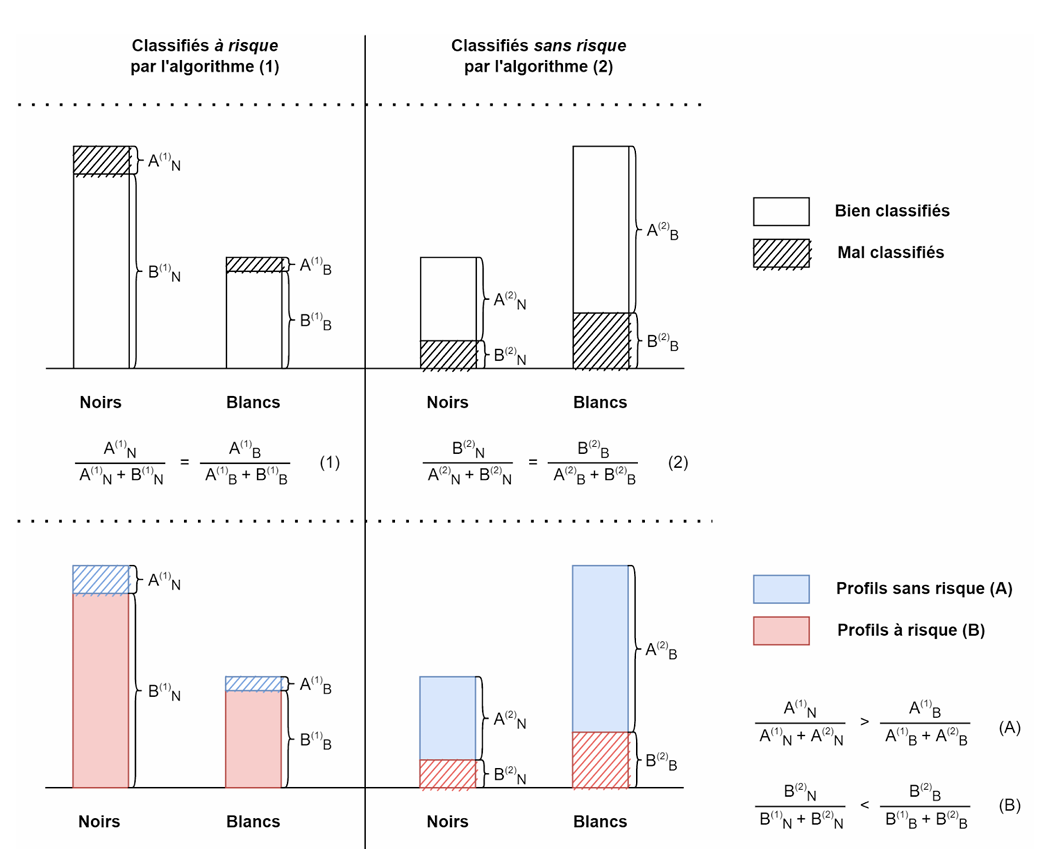
\includegraphics[width=0.5\linewidth]{images/Graphique COMPAS.PNG}
    \caption{Différences de couleurs des profils pourtant similaires considérés à risque ou non d'après l'algorithme de COMPAS\cite{noauthor_compas_nodate}}
    \label{COMPAS graph}
\end{figure}
Il en va de même avec les programmes de reconnaissance faciale et d'identification de l'orientation sexuelle qui, mal codés conformément à l'éthique, peuvent porter atteinte à certains groupes de personnes.\\
\\ Ce sont des choses déjà vues en cours, mais qui, je pense, ont totalement leur place dans ce sujet.\\
\\ Produire des logiciels ne possédant pas un code éthique est aussi problématique que dangereux pour les développeurs et les utilisateurs.\\\\

 Tout d'abord des discriminations raciales qui vont donc à l'encontre des lois françaises, comme j'ai pu le dire plus tôt avec l'exemple de l'IA COMPAS aux États-Unis, le danger est aussi pour la planète, un code non éthique et non optimisé entraînera un certain impact sur l'environnement ce qui sera étudié en profondeur par Lynne.\\\\

Ensuite un code non éthique peut être défavorable pour certaines personnes; certains algorithmes codés sans contraintes éthiques finissent par être problématiques et peuvent entraîner des discriminations pour les personnes handicapées par exemple, ce que Sephora mettra en lumière dans sa partie.\\\\

Enfin le manque de protection peut mettre en danger les informations personnelles des utilisateurs et les laisser fuiter entre les mains des personnes mal intentionnées. C'est ici que la cybersécurité joue une place importante pour assurer la conformité d'un code, pour éviter que ce genre d'événements se produise comme l'expliquera Andrea. Dans le même cas, les utilisateurs ne feront plus confiance à ces logiciels, ce qui mettra donc en péril le travail des développeurs et la réputation de l'entreprise derrière.\\

\subsection{L'impact sur l'environnement, et les des droits des travailleurs (Lynne)} 
Puisqu’on parle d’éthique, il nous paraît parfaitement pertinent de traiter la question de l’impact du code sur l’environnement, ainsi que celle des droits des travailleurs dans le domaine.\\ 

On pourrait reprocher plusieurs choses aux cryptomonnaies, par exemple, le fait qu’elles facilitent le blanchiment d’argent et qu’il s’agit d’une forme d’investissement pas tout à fait infaillible, mais surtout leur impact écologique désastreux. On estime que la consommation électrique annuelle dédiée au minage du bitcoin est comparable à celle de la Pologne, et pour ce qui est de l’empreinte hydrique, les scientifiques estiment qu'elle est équivalente à celle de 660 000 piscines olympiques (pour la période entre janvier 2020 et décembre 2021), soit environ 800 milliards de litres par an. Il est important de mentionner aussi que de petites inefficacités dans le code (hors-blockchain, hors-cryptomonnaie) peuvent s’accumuler et entraîner des retards importants qui augmentent la consommation d'électricité et les coûts de fonctionnement, surtout si un logiciel ou un service possède un grand nombre d’utilisateurs. Ce phénomène est davantage polluant si on tient compte du fait que si l’on héberge du code sur AWS (Amazon Web Services), cela implique l’exploitation des énergies fossiles, AWS étant le plus grand fournisseur de cloud computing.\\

Il y a 2 facteurs qui font que les LLMs sont extrêmement énergivores : leur utilisation et leur entraînement. Une conversation moyenne avec ChatGPT consomme approximativement 500 ml d’eau, des impacts considérables si l’on compte les 1,5 milliard d’utilisateurs mensuels. Les data centers sont également fortement gourmands en énergie. En 2023, l’Agence internationale de l’énergie a révélé que les centres de données représentent environ 1 à 1,5\% de la consommation électrique mondiale. Ces chiffres risquent de s'accentuer à cause de la hausse croissante de la demande. La phase de pré-entraînement de GPT-3 a généré l’équivalent de 626 000 kg de CO₂, soit 71.9 tours de la terre en voiture ou la fabrication de 3 244 ordinateurs portables. (Source : Comparateur Carbone)\\

D’ailleurs, l’IA n’est pas réellement de l’Intelligence Artificielle à proprement parler, c’est une approximation de l’intelligence humaine. Un GML n’est pas capable de raisonner, ce qui rend l’automatisation complète impossible selon Antonio A. Casilli, comme il l’explique dans son livre “En Attendant Les Robots”. Les “travailleurs du clic”, donc, “toute personne qui annote, filtre, enrichit ou structure des données pour la création d’énormes bases de données” sont, pour la plupart, issus des pays du sud global, et sont extrêmement sous-payés. Ces travailleurs sont invisibilisés et absents des textes régulant l’Intelligence Artificielle, même au sein de l’IA Act. Cette même main d’œuvre subit actuellement une forme d’expulsion massive (Personnes issues des pays de l’Amérique Latine aux É.-U.), alors que la même administration à l’avant-garde de la déréglementation massive de l’IA continue de les exploiter pour s’enrichir, tout en les mettant à l’écart.\\ 


L’éthique ne concerne pas seulement la manière dont on écrit le code, mais aussi la manière dont on traite les ouvriers.\\ 

\subsection{Le manque d'accessibilité pour les personnes déficientes visuellement (Sephora)}

Un manque d’éthique inclusive réduit l’accès à des logiciels, certaines mesures adaptatives mises en place pour les personnes malvoyantes/aveugles peuvent avoir des retombées positives pour les autres utilisateurs qui n’ont pas de déficiences visuelles. \\ \\
Le plan d’action eEurope 2005 promouvait l’e-inclusion mais certains logiciels utilisés pour le réaliser étaient incompatibles avec les narrateurs de lecture d'écran (qui sont des dispositifs d’assistance destinés aux personnes aveugles) après la mise en service de nouveaux systèmes d'exploitation. Ce qui peut être perçu comme un manque de valorisation des besoins des personnes victimes de déficience visuelles dans l’éthique que l’on suit lors de la création d’un logiciel. 
\\\\
L’intégration de dispositif d’assistance n’est plus uniquement basée sur son bon vouloir mais elle est maintenant règlementée. En effet elle est réglementée par le W3C qui crée des standards et des lignes directrices à suivre lors de la création des technologies Web dans le monde. 
\\\\
En France L’association \cite{Wikipedia}.BrailleNet (liquidée judiciairement depuis 2022) décernait un label AccessiWeb qui certifiait de l’accessibilité des logiciels ou sites web sur demande de leurs responsables. Cette association a notamment été membre du W3C et a participé à la traduction française du WCAG (Web Content Accessibility Guidelines). 
\\\\
AccessiWeb a aussi contribué à la formation de 1500 experts à l’accessibilité numérique (2014) ce qui montre une réelle démarche pour l’évolution de l’accessibilité. 
\\\\
\cite{Gourvennec_2024}Au niveau de la législation française Pierre Marragou a assigné en justice l’État en justice pour ne pas avoir respecté une des lois du plan d’action eEurope 2005 pendant 19 ans. Dans les faits depuis l’instauration de cette loi qui cherchais à promouvoir l’accessibilité des logiciels de vie scolaire ne la respectaient pas ce qui empêchais les élèves ou parents malvoyants de l’utiliser. \\ Malgré la contestation de Sophie Cluzel (secrétaire de l’état) le jugement qui a été rendu oblige l’ARCOM, à mettre en œuvre ses pouvoirs pour vérifier si, oui ou non, les logiciels de vie scolaire sont conformes aux normes d’accessibilité. \\\\ 
Enfin certains dispositifs de vérification comme les Captchas \cite{Wagner_2022b} peuvent êtres des entraves semées sur le chemin des personnes malvoyantes. Ils peuvent enlever ce côté pratique qu’a internet de pouvoir disposer et effectuer certaines tâches plus facilement pour les personne aveugle à cause de ce système de validation anti-robot qui repose majoritairement sur des tests visuels. \\\\

\subsection{Protection des Données et Vie Privée (Andrea)}

L’éthique au sein du développement des logiciels concerne également la protection de la vie privée, un enjeu fondamental. En intégrant des mesures de protection dès la phase de conception des applications, on assure une sécurité optimale des données personnelles des utilisateurs. Cette approche, appelée « Protection de la vie privée dès la conception » (Privacy by Design), se construit autour de plusieurs principes clés comme l’anticipation des violations de la vie privée, la sécurisation et protection de cette dernière ou encore la transparence totale des actions faites par ce logiciel.
\\\\
 La mise en œuvre de ces principes durant le développement des logiciels permet non seulement de se conformer aux réglementations en vigueur, comme le Règlement Général sur la Protection des Données (RGPD) en Europe, mais également de renforcer la confiance des utilisateurs envers les produits et services proposés. En intégrant la protection de la vie privée dès la conception, les développeurs œuvrent pour un environnement numérique plus sûr et respectueux des droits individuels.
\\\\
 Il faut savoir également qu’un certain nombre de logiciels espions sont sur le marché, ces logiciels bien qu’au départ conçus pour un contrôle parental, sont utilisés à des fins illégales (en France) pour espionner son conjoint ou ses proches. Ces logiciels espions sont très faciles d’accès et malheureusement, rien n’existe actuellement pour empêcher les ordinateurs et téléphones d’être contrôlés par ces logiciels invisibles à l’œil des consommateurs.
\\\\
Il est aussi fondamental de prendre en compte les utilisateurs vivant dans des pays autoritaires, c’est-à-dire qu’il ne faut pas laisser des failles de sécurité qui permettraient à ces gouvernements de pister leurs citoyens, les empêchant d’exercer leur liberté d’expression. Cela conduit bon nombre d’entre eux à utiliser des VPN ou « Virtual Private Network », des logiciels conçus pour sécuriser les connexions publiques mais qui dans ces cas-là, permet à ces citoyens de bénéficier d’un internet libre et non-surveillé par les autorités locales, en passant outre les interdictions du pays en question. Le sujet de l’autoritarisme évoque évidemment les logiciels de surveillance, tels que les logiciels de reconnaissance faciale, entre autres. En Pologne, l’utilisation du logiciel “Pegasus” a fait partie d’un "système de surveillance de l'opposition et des voix critiques vis-à-vis du gouvernement, conçu pour maintenir la majorité dirigeante et le gouvernement au pouvoir", selon le Parlement Européen. On vit actuellement dans un contexte politique très tendu, où les droits de nombreuses minorités ainsi que la démocratie sont menacés, ce qui fait qu’il est essentiel de penser à toutes les manières dont un logiciel pourrait être utilisé pour nuire aux libertés fondamentales des utilisateurs.\\

\subsection{Conclusion}
En guise de conclusion, on peut dire qu’il faut absolument prendre conscience des enjeux éthiques lors de la création de logiciels, qui, eux, sont présents à chaque phase du développement, et peuvent toucher plusieurs secteurs de la population: quelques algorithmes vont, par exemple, refléter les biais de la société dans laquelle ils ont été créés (COMPAS) et, ce faisant, enfreindre certaines lois de non-discrimination, tandis que d’autres algorithmes/programmes qui ne répondent pas forcément à un besoin humain essentiel (cryptomonnaies) auront un impact désastreux sur l’environnement. De graves fautes en matière d’éthique peuvent aussi être commises à l’égard des droits des travailleurs, ou encore de manière moins intentionnelle envers les personnes en situation de handicap, en les tenant à l’écart du monde numérique par le biais des CAPTCHAs, par exemple. Dernier point, mais pas le moindre, le respect de la vie privée et des libertés humaines fondamentales constitue, lui aussi, un enjeu éthique crucial. \\


\subsection{Retour Réflexif}


\bibliographystyle{unsrt}

\bibliography{Sources}

\end{document}